\documentclass{book}
\usepackage[subpreambles=false]{standalone}

%%%%%%%%%%%%%%%%%%%%%%%%%%%
% Silence warning messages
\usepackage{silence}
\WarningsOff[scrlayer-notecolumn]
\WarningsOff[biblatex]

%%%%%%%%%%%%%%%%%%%%
% Commenting

%\usepackage[author=Lyndon]{pdfcomment}
%\newcommand{\pdfcomment}[1]{} %ignore all comments

%\usepackage{todonotes}
%\newcommand{\pdfcomment}{\todo}


%%%%%%%%%%%%%%%%%%%%
% Tables
\usepackage{booktabs}

%%%%%%%%%%%%%%%%%%%
% Fonts
\usepackage{tgadventor} %sans
\usepackage{tgpagella}  %serif
\usepackage{inconsolata} %mono
\usepackage[T1]{fontenc}

\usepackage{microtype}
\usepackage[all]{nowidow}
%%%%%%%%%%%%%%%%%%%%%%%
% Styling
\setcounter{secnumdepth}{4}
\setcounter{tocdepth}{2}

\usepackage{placeins}



%%%%%%%%%%%%%%%%%%%
% Math
\usepackage{amsmath, amssymb, stmaryrd, mathtools}
\DeclareMathOperator*{\argmin}{argmin}
\DeclareMathOperator*{\argmax}{argmax}

\usepackage{xparse,xstring,etoolbox}
% crossref this against notation section
\newcommand{\vv}[1]{\tilde{#1}} % vector
\newcommand{\seq}[1]{\mathcal{#1}} % sequence
\newcommand{\set}[1]{\mathbb{#1}} % set

%%%%%%%%%
% Indexing/sequence indexing
\newcommand{\seqind}[2]{#1^{#2}} % seqence index
\newcommand{\ind}[2]{#1_{#2}} % indexed
\newcommand{\disamb}[2]{#1^{\mathrm{#2}}} %disambiguated

%% Smart indexing and naming
\newcommand{\ifupper}[3]{
    \normalexpandarg
	\exploregroups
	\StrCount{ABCDEFGHIJKLMNOPQRSTUVWXYZ}{#1}[\uppercount]
	\ifnumgreater{\uppercount}{0}{#2}{#3}
}

%smart index
\DeclareDocumentCommand{\ii}{u{_} m}{
	\ifupper{#1}%
	{% just a single uppercase character, i.e. a matrix
		  %make sure the index is the right length
		\StrCount{#2}{,}[\indcount]
		\ifnumgreater{\indcount}{0}
		{ % Got multiple indexes so all good
		 	\ind{#1}{#2}
		}
		{ % Only 1 index so grab the column
		 	\ind{#1}{{:,#2}}
		}
	}%
	{% Not just a single upper case character
		\ind{#1}{#2}
	}
}

\DeclareDocumentCommand{\nn}{u{_} m}{
	\seqind{#1}{#2}
}

\DeclareDocumentCommand{\dd}{u{_} m}{
	\disamb{#1}{#2}
}

% Index of a vector
\DeclareDocumentCommand{\iv}{u{_} m}{\ii{\vv #1}_{#2}}
\DeclareDocumentCommand{\dv}{u{_} m}{\dd{\vv #1}_{#2}}
\DeclareDocumentCommand{\nv}{u{_} m}{\nn{\vv #1}_{#2}}

%exp
\let\oldexp\exp
\renewcommand{\exp}[1]{\oldexp \left( #1 \right)}
\newcommand{\exptwo}[1]{\oldexp_2 \left( #1 \right)}

\newcommand{\softmax}{\mathrm{smax}}

\DeclareMathOperator*{\expectedop}{\mathbb{E}}
\DeclareDocumentCommand{\expected}{u{_} m}{
	\expectedop\limits_{\mathrlap{#2}}
}

%%%%%%%%%%%%%%%%
%Graphics
\usepackage{tikz}
\usetikzlibrary{positioning, fit,  shapes.geometric}
\usepackage{ifthen}
\usepackage{etoolbox}

\tikzset{
	backgroundcolor/.style ={fill=white},
	every node/.append style={
		minimum height=7mm,
	},
	labe/.append style={
		%Blue,
		align = center,
		backgroundcolor,
		fill opacity=0.6,
		text opacity=1,
		font={\footnotesize\itshape}	
	},
	layer/.append style={
		draw,
		align = center,
		minimum height=7mm,
	},
	tight/.append style={
		inner sep=0.2mm,
	},
	lookupbox/.append style={
		draw=none,
		append after command={
		       	[shorten <= -0.5\pgflinewidth]
		       	([shift={(-1.5\pgflinewidth,-0.5\pgflinewidth)}]\tikzlastnode.north east)
		       	edge([shift={( 0.5\pgflinewidth,-0.5\pgflinewidth)}]\tikzlastnode.north west) 
		       	([shift={( 0.5\pgflinewidth,-0.5\pgflinewidth)}]\tikzlastnode.north west)
		       	edge([shift={( 0.5\pgflinewidth,-1.5\pgflinewidth)}]\tikzlastnode.south west)            
		       	([shift={( -1.5\pgflinewidth,+0.5\pgflinewidth)}]\tikzlastnode.south east)
		       	edge([shift={(-1.5\pgflinewidth,-0.5\pgflinewidth)}]\tikzlastnode.north east)
		},
		inner sep=0.7mm,
		outer sep=0mm,
		minimum width=25mm
	}
}

\usepackage{pgfplots}
\pgfplotsset{compat=1.14}
\pgfplotsset{sideplot/.append style={
		width=\notescolwidth,
		domain=-10:10,
		samples=101,
		smooth,
		enlarge y limits={abs=2},
		axis lines=middle,
		xlabel  = $z$,
		ylabel  = $y$,
	},
	equ/.append style={
		color=blue,
		thick,
		mark=none
	}
}

% Function  For a plot 
% it  needs to be declared in preamble because of how \makenote* interacts with multiple files
\def\errorsurface(#1,#2){(0.5*#1 + 0.7*#2 + sin(deg(1.5*#1 + #2^2)))^2}


\usepackage{graphicx}
\graphicspath{{./figs/}, {./}, {./figs/chaptersentencerrepr/}, {./figs/chapterintromachinelearning/}, {./figs/chapterwordrepr/}}
\usepackage{adjustbox}


%%%%%%%%%%%%%%%%%%%
% Refs
\usepackage{cleveref}

\addbibresource{master.bib}

%%%%%%%%%%%%%%%%%%%%
% Formatting

% for examples from natural language space.
\newcommand{\natlang}[1]{\ifmmode \text{``\texttt{#1}''} \else {``\texttt{#1}''}\fi}
% \ifmmode ``trick'' from https://tex.stackexchange.com/a/15194/5834

%%%%%%%%%%%%%%%%%%%%%



\begin{document}
	
\chapter{Conclusion}
The research presented here on linear combinations of embeddings has highlighted an interesting fact.
It has been shown that this simple input representation technique is surprisingly powerful.
This surprising power come from the value of surface level information in many practical natural language understanding tasks.
The word content being the most obvious of these.
This word content is presented in a dense and informative form in a LCOWE; in a way that captures and preserves lexical similarity information.
While the LCOWE loses word order information, it very well preserves the word content.
That content proved more useful for the tasks considered in this research.


Future work in this area requires not just the construction of adversarial examples; but of the determination of how common they are in practice.
Adversarial examples are not ubiquitous in real world tasks.
It is important not to succeed on only these cases, while failing on the more common simple cases.

It is also important to consider how adversarial such a challenging case is.
In \Cref{ColorEst}, the ordered task which was to make predictions for colors for which the different words in the name could appear in different orders to describe different colors.
For example \natlang{bluish green} and \natlang{greenish blue} are different colors.
However, they are very \emph{similar} colors.
As such the error from discarding word order, is less than the error from using a more complicated model such as an RNN.
Such a more complex model is harder to train, and those practical difficulties can dominate over a small amount of theoretical lack of capacity.


There is a complementary aspect to LCOWE and language models.
While LCOWE have no capacity to handle word order but excellent ability to capture word content;
Pure language models have no ability to capture word content, but excellent ability to capture word order.
Language modelling based tasks incorporating a representation stage, such as encoder-decoders \citep{cho-EtAl:2014:EMNLP2014}, do not capture word content as well as LCOWE \citep{ac2018probingsentencevectors}.
They do, however, have state of the art order order representation.
\todo{I would really like to talk about how word embeddings are useful for caption evaluation here.}

Future work in this area would be to enhance an encoder-decode model by concatenating to the shared state a SOWE.
\todo{REDO this figure with the Embedding layers shown and the SOWE shared representation laye radded}



\begin{figure}
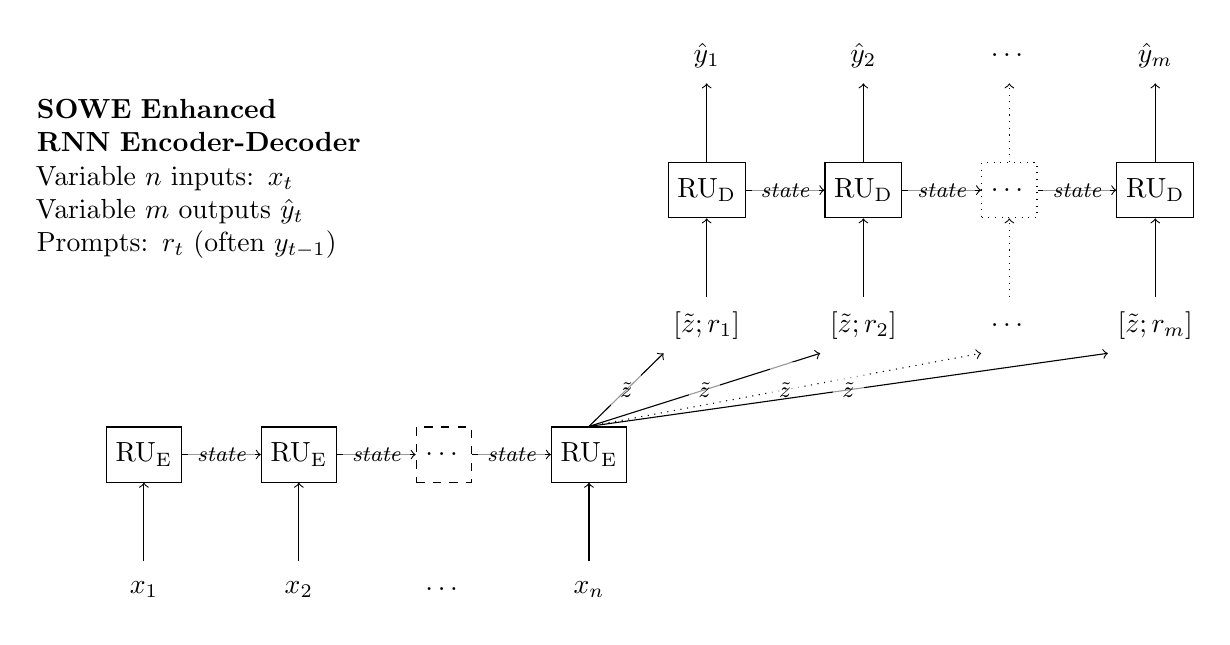
\begin{tikzpicture}
	\numdef{\N}{8}
	\numdef{\labelwidth}{5.5cm}

	\node(lbl)[text width= \labelwidth] {\textbf{SOWE Enhanced\\RNN Encoder-Decoder}\\%
		Variable $n$ inputs: $\nv x_t$\\%
		Variable $m$ outputs $\nn \hat{y}_t$\\%
		Prompts: $\nv r_t$ (often $y_{t-1}$)
	};
	
	\coordinate[yshift = -3.5cm] (L0) at (lbl.west);
	\numdef{\NN}{4}
	\foreach \I[count=\j from 0] in {1,...,\NN}{
		\ifnumequal{\I}{\NN - 1}{%
			\node(L\I)[dashed, layer, right = of L\j] {\ldots};
			\node(w\I)[below = of L\I]{\ldots};
		}%
		{
			\node(L\I)[layer, right = of L\j] {$\mathrm{RU_E}$};
			\node(w\I)[below = of L\I]{\ifnumequal{\I}{\NN}{$\nv x_n$}{$\nv x_\I$}};
			\draw[->] (w\I) -- (L\I);
		}
	}
	\foreach \I[count=\j from 1] in {2,...,\NN} {
		\draw[->] (L\j) edge node[labe] {state} (L\I);
	}
	
	
	
	
	\coordinate[above = 3 of L\NN] (Lp\NN);
	\numdef{\NP}{\N - 1}
	\foreach \j in {\NN,...,\NP}{
		\numdef{\I}{\j+1}
		\numdef{\y}{\I - \NN}
		\ifnumequal{\I}{\N-1}{%
			\node(Lp\I)[dotted, layer, right = of Lp\j] {\ldots};
			\node(w\I)[below = of Lp\I]{\ldots};
			\node(y\I)[above = of Lp\I]{\ldots};
			\draw[->,dotted] (w\I) -- (Lp\I);
			\draw[->,dotted] (Lp\I) -- (y\I);
			\path[->,dotted] (L\NN.north) edge node[labe]{$\vv z$} (w\I.south west);
		}%
		{
			\node(Lp\I)[layer, right = of Lp\j] {$\mathrm{RU_D}$};
			\ifnumequal{\I}{\N}{
				\node(w\I)[below = of Lp\I]{$[\vv z; \nv r_m]$};
				\node(y\I)[above = of Lp\I]{$\nn \hat{y}_m$};
			}
			{
				\node(w\I)[below = of Lp\I]{$[\vv z; \nv r_\y]$};
				\node(y\I)[above = of Lp\I]{$\nn \hat{y}_\y$};
			}
			
			\draw[->] (w\I) -- (Lp\I);
			\draw[->] (Lp\I) -- (y\I);
			\path[->] (L\NN.north) edge node[labe]{$\vv z$} (w\I.south west);
		}
	}
	
	
	\numdef{\NNp1}{\NN + 1}
	\foreach \I in {\NNp1,...,\NP} {
		\numdef{\j}{\I+1}
		\draw[->] (Lp\I) edge node[labe] {state} (Lp\j);
	}
\end{tikzpicture}

\end{figure}



\section{Some reflections upon semantic spaces}
\begin{figure}
	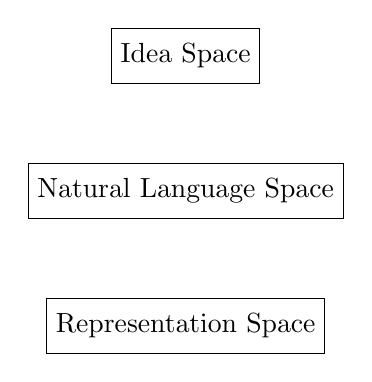
\begin{tikzpicture}
		\node[draw](idea){Idea Space};
		% Objects: ideas, thoughts
		\node[draw, below = of idea](nl){Natural Language Space};
		% Objects: utterances, sentences, words
		\node[draw, below = of nl](emb){Representation Space};
		% Objects: Embeddings
	\end{tikzpicture}
\end{figure}

We can consider that there is a true semantic space of ideas that we try to recover when we try and understand something's meaning.
When speaking, this space is projected down to natural languages space.
To again quote Webber: ``A sentence is a group of words expressing a complete thought.''.
This projection is imperfect -- it is lossy.
Some times the natural language space alone, is enough to recover a good idea of the the point in idea space the speaker intends,
but other times it is not.
Instead, we can end up with the 


The preimage of a point in natural language space (e.g. a sentence),
is a probability distribution over idea space that could have lead to that utterance -- $P(meaning \mid utterance)$.
This distribution could be combined with other factors (in a Baysian way); either from that natural language context, or the enviroment more broadly.
For example, to use a meaning that centres around word sense:
we can identify two (of the many) senses of the word \natlang{apples}:
one in reference to the fruit, the other in reference to the computers made by the eponymous company.
Thus, on its own the sentence \natlang{Apples are good.}
suggests a distribution with at least two peaks in idea space.
Combine that utterance, with the context of being in a computer store, rather than a grocer, and the probability of one peak can be increased, though  the other not entirely removed.
Further around each peak remains adjacent closely related possible meanings.
For example the statement could be in relation to only computers, or also to other products.
idea space is a continuous space, with every utterance corresponding to a unique point. It is an uncountably large space.
In contrast natural language space is countably large, being composed of finite length combinations of of symbols taken from a finite alphabet.
An uncountable number of points in idea space are projected down to a single point in natural language space.




When designing a embedding method, for sentences, words or other structures,
we seek to define a representation space
that has good 
In particular it should have a continuous mapping from to and from embedding space.
A neighbourhood in representation space, should correspond to a neighbourhood in idea space.
\Cref{SentVecMeaning} investigated this for sentence embeddings.
By taking points in natural language space known to come from very near by points in idea space, that is to say paraphrases,
and checking that they belong to near points in embedding space.


As each point in natural language space is defines a distribution over idea space of what may be meant;
and representation space is attempting to be in correspondence to idea space;
it is such that each point in natural language space should project to a distribution over embedding space.
Instead, most methods project to natural language points to single points in embeddings space.
This is viable when the region in idea space that the natural language point could have come from is small -- in particular that the distribution in idea space is narrow variance and mono-modal.
In that case the single point estimate in embedding space is an useful approximation.


In the case of words with multiple meanings, 
word-sense embeddings produce multiple sense embeddings -- ideally one corresponding to each peak in idea space.
We know these peaks are only rough approximations to the true point in idea space for a given usage of a word.
\Cref{RefittingSenses} attempts find other points in the embeddings space, that better corresponds to the true point in idea space for the particular use.


Unsupervised methods, in particular word embeddings, but also more generally, are ungrounded.
They found on principles such as Firth's distributional hypothesis:
that word occurring in similar contexts have similar meaning. 
The goal is not to capture I meaning in this space,
but rather to create a space that is a good input to a supervised system that can learn a good correspondence from natural language space to idea space. 

The color understanding task considered in \Cref{ColorDist} is interesting.
While it is a typical natural language understanding system,
which takes a point in natural language space (a color name),
moves through a representation space (the output of one of the input modules: SOWE, CNN, or RNN) using supervision to output something from meaning space.
In this case the meaning space is explicit, it is the HSV color space.
Using point estimation it outputs a point in meaning space













\printbib


\end{document}